% Created by tikzDevice version 0.10.1 on 2016-08-26 10:18:06
% !TEX encoding = UTF-8 Unicode
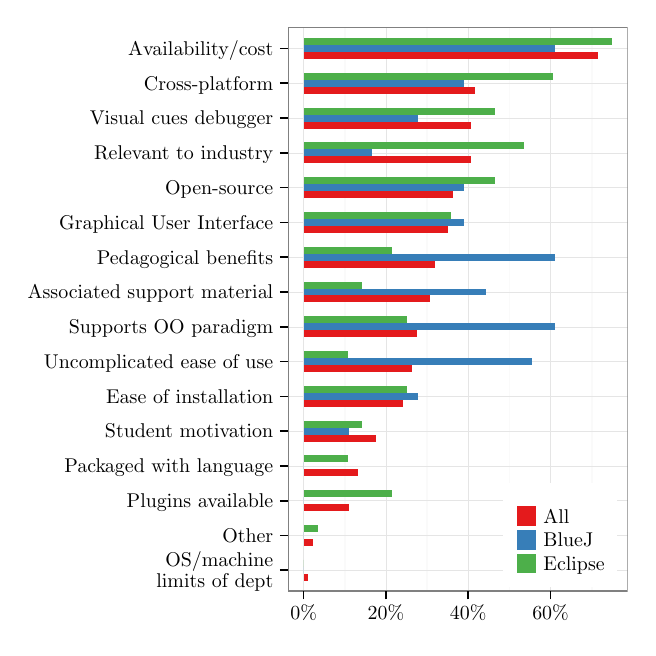
\begin{tikzpicture}[x=1pt,y=1pt]
\definecolor{fillColor}{RGB}{255,255,255}
\path[use as bounding box,fill=fillColor,fill opacity=0.00] (0,0) rectangle (216.81,216.81);
\begin{scope}
\path[clip] (  0.00,  0.00) rectangle (216.81,216.81);
\definecolor{drawColor}{RGB}{255,255,255}
\definecolor{fillColor}{RGB}{255,255,255}

\path[draw=drawColor,line width= 0.6pt,line join=round,line cap=round,fill=fillColor] (  0.00,  0.00) rectangle (216.81,216.81);
\end{scope}
\begin{scope}
\path[clip] ( 94.14, 13.20) rectangle (216.81,216.81);
\definecolor{fillColor}{RGB}{255,255,255}

\path[fill=fillColor] ( 94.14, 13.20) rectangle (216.81,216.81);
\definecolor{drawColor}{gray}{0.98}

\path[draw=drawColor,line width= 0.6pt,line join=round] (114.58, 13.20) --
	(114.58,216.81);

\path[draw=drawColor,line width= 0.6pt,line join=round] (144.32, 13.20) --
	(144.32,216.81);

\path[draw=drawColor,line width= 0.6pt,line join=round] (174.06, 13.20) --
	(174.06,216.81);

\path[draw=drawColor,line width= 0.6pt,line join=round] (203.80, 13.20) --
	(203.80,216.81);
\definecolor{drawColor}{gray}{0.90}

\path[draw=drawColor,line width= 0.2pt,line join=round] ( 94.14, 20.75) --
	(216.81, 20.75);

\path[draw=drawColor,line width= 0.2pt,line join=round] ( 94.14, 33.31) --
	(216.81, 33.31);

\path[draw=drawColor,line width= 0.2pt,line join=round] ( 94.14, 45.88) --
	(216.81, 45.88);

\path[draw=drawColor,line width= 0.2pt,line join=round] ( 94.14, 58.45) --
	(216.81, 58.45);

\path[draw=drawColor,line width= 0.2pt,line join=round] ( 94.14, 71.02) --
	(216.81, 71.02);

\path[draw=drawColor,line width= 0.2pt,line join=round] ( 94.14, 83.59) --
	(216.81, 83.59);

\path[draw=drawColor,line width= 0.2pt,line join=round] ( 94.14, 96.15) --
	(216.81, 96.15);

\path[draw=drawColor,line width= 0.2pt,line join=round] ( 94.14,108.72) --
	(216.81,108.72);

\path[draw=drawColor,line width= 0.2pt,line join=round] ( 94.14,121.29) --
	(216.81,121.29);

\path[draw=drawColor,line width= 0.2pt,line join=round] ( 94.14,133.86) --
	(216.81,133.86);

\path[draw=drawColor,line width= 0.2pt,line join=round] ( 94.14,146.43) --
	(216.81,146.43);

\path[draw=drawColor,line width= 0.2pt,line join=round] ( 94.14,159.00) --
	(216.81,159.00);

\path[draw=drawColor,line width= 0.2pt,line join=round] ( 94.14,171.56) --
	(216.81,171.56);

\path[draw=drawColor,line width= 0.2pt,line join=round] ( 94.14,184.13) --
	(216.81,184.13);

\path[draw=drawColor,line width= 0.2pt,line join=round] ( 94.14,196.70) --
	(216.81,196.70);

\path[draw=drawColor,line width= 0.2pt,line join=round] ( 94.14,209.27) --
	(216.81,209.27);

\path[draw=drawColor,line width= 0.2pt,line join=round] ( 99.71, 13.20) --
	( 99.71,216.81);

\path[draw=drawColor,line width= 0.2pt,line join=round] (129.45, 13.20) --
	(129.45,216.81);

\path[draw=drawColor,line width= 0.2pt,line join=round] (159.19, 13.20) --
	(159.19,216.81);

\path[draw=drawColor,line width= 0.2pt,line join=round] (188.93, 13.20) --
	(188.93,216.81);
\definecolor{fillColor}{RGB}{228,26,28}

\path[fill=fillColor] ( 99.71, 16.97) rectangle (101.35, 19.49);
\definecolor{fillColor}{RGB}{77,175,74}

\path[fill=fillColor] ( 99.71, 22.00) rectangle ( 99.71, 24.52);
\definecolor{fillColor}{RGB}{55,126,184}

\path[fill=fillColor] ( 99.71, 19.49) rectangle ( 99.71, 22.00);
\definecolor{fillColor}{RGB}{228,26,28}

\path[fill=fillColor] ( 99.71, 29.54) rectangle (102.99, 32.06);
\definecolor{fillColor}{RGB}{77,175,74}

\path[fill=fillColor] ( 99.71, 34.57) rectangle (105.02, 37.08);
\definecolor{fillColor}{RGB}{55,126,184}

\path[fill=fillColor] ( 99.71, 32.06) rectangle ( 99.71, 34.57);
\definecolor{fillColor}{RGB}{228,26,28}

\path[fill=fillColor] ( 99.71, 42.11) rectangle (116.06, 44.62);
\definecolor{fillColor}{RGB}{77,175,74}

\path[fill=fillColor] ( 99.71, 47.14) rectangle (131.58, 49.65);
\definecolor{fillColor}{RGB}{55,126,184}

\path[fill=fillColor] ( 99.71, 44.62) rectangle ( 99.71, 47.14);
\definecolor{fillColor}{RGB}{228,26,28}

\path[fill=fillColor] ( 99.71, 54.68) rectangle (119.33, 57.19);
\definecolor{fillColor}{RGB}{77,175,74}

\path[fill=fillColor] ( 99.71, 59.71) rectangle (115.64, 62.22);
\definecolor{fillColor}{RGB}{55,126,184}

\path[fill=fillColor] ( 99.71, 57.19) rectangle ( 99.71, 59.71);
\definecolor{fillColor}{RGB}{228,26,28}

\path[fill=fillColor] ( 99.71, 67.25) rectangle (125.85, 69.76);
\definecolor{fillColor}{RGB}{77,175,74}

\path[fill=fillColor] ( 99.71, 72.27) rectangle (120.96, 74.79);
\definecolor{fillColor}{RGB}{55,126,184}

\path[fill=fillColor] ( 99.71, 69.76) rectangle (116.23, 72.27);
\definecolor{fillColor}{RGB}{228,26,28}

\path[fill=fillColor] ( 99.71, 79.82) rectangle (135.67, 82.33);
\definecolor{fillColor}{RGB}{77,175,74}

\path[fill=fillColor] ( 99.71, 84.84) rectangle (136.89, 87.36);
\definecolor{fillColor}{RGB}{55,126,184}

\path[fill=fillColor] ( 99.71, 82.33) rectangle (141.02, 84.84);
\definecolor{fillColor}{RGB}{228,26,28}

\path[fill=fillColor] ( 99.71, 92.38) rectangle (138.92, 94.90);
\definecolor{fillColor}{RGB}{77,175,74}

\path[fill=fillColor] ( 99.71, 97.41) rectangle (115.64, 99.93);
\definecolor{fillColor}{RGB}{55,126,184}

\path[fill=fillColor] ( 99.71, 94.90) rectangle (182.33, 97.41);
\definecolor{fillColor}{RGB}{228,26,28}

\path[fill=fillColor] ( 99.71,104.95) rectangle (140.56,107.47);
\definecolor{fillColor}{RGB}{77,175,74}

\path[fill=fillColor] ( 99.71,109.98) rectangle (136.89,112.49);
\definecolor{fillColor}{RGB}{55,126,184}

\path[fill=fillColor] ( 99.71,107.47) rectangle (190.58,109.98);
\definecolor{fillColor}{RGB}{228,26,28}

\path[fill=fillColor] ( 99.71,117.52) rectangle (145.47,120.03);
\definecolor{fillColor}{RGB}{77,175,74}

\path[fill=fillColor] ( 99.71,122.55) rectangle (120.96,125.06);
\definecolor{fillColor}{RGB}{55,126,184}

\path[fill=fillColor] ( 99.71,120.03) rectangle (165.79,122.55);
\definecolor{fillColor}{RGB}{228,26,28}

\path[fill=fillColor] ( 99.71,130.09) rectangle (147.10,132.60);
\definecolor{fillColor}{RGB}{77,175,74}

\path[fill=fillColor] ( 99.71,135.12) rectangle (131.58,137.63);
\definecolor{fillColor}{RGB}{55,126,184}

\path[fill=fillColor] ( 99.71,132.60) rectangle (190.58,135.12);
\definecolor{fillColor}{RGB}{228,26,28}

\path[fill=fillColor] ( 99.71,142.66) rectangle (151.99,145.17);
\definecolor{fillColor}{RGB}{77,175,74}

\path[fill=fillColor] ( 99.71,147.68) rectangle (152.81,150.20);
\definecolor{fillColor}{RGB}{55,126,184}

\path[fill=fillColor] ( 99.71,145.17) rectangle (157.54,147.68);
\definecolor{fillColor}{RGB}{228,26,28}

\path[fill=fillColor] ( 99.71,155.23) rectangle (153.63,157.74);
\definecolor{fillColor}{RGB}{77,175,74}

\path[fill=fillColor] ( 99.71,160.25) rectangle (168.75,162.77);
\definecolor{fillColor}{RGB}{55,126,184}

\path[fill=fillColor] ( 99.71,157.74) rectangle (157.54,160.25);
\definecolor{fillColor}{RGB}{228,26,28}

\path[fill=fillColor] ( 99.71,167.79) rectangle (160.17,170.31);
\definecolor{fillColor}{RGB}{77,175,74}

\path[fill=fillColor] ( 99.71,172.82) rectangle (179.37,175.33);
\definecolor{fillColor}{RGB}{55,126,184}

\path[fill=fillColor] ( 99.71,170.31) rectangle (124.50,172.82);
\definecolor{fillColor}{RGB}{228,26,28}

\path[fill=fillColor] ( 99.71,180.36) rectangle (160.17,182.88);
\definecolor{fillColor}{RGB}{77,175,74}

\path[fill=fillColor] ( 99.71,185.39) rectangle (168.75,187.90);
\definecolor{fillColor}{RGB}{55,126,184}

\path[fill=fillColor] ( 99.71,182.88) rectangle (141.02,185.39);
\definecolor{fillColor}{RGB}{228,26,28}

\path[fill=fillColor] ( 99.71,192.93) rectangle (161.81,195.44);
\definecolor{fillColor}{RGB}{77,175,74}

\path[fill=fillColor] ( 99.71,197.96) rectangle (189.99,200.47);
\definecolor{fillColor}{RGB}{55,126,184}

\path[fill=fillColor] ( 99.71,195.44) rectangle (157.54,197.96);
\definecolor{fillColor}{RGB}{228,26,28}

\path[fill=fillColor] ( 99.71,205.50) rectangle (205.93,208.01);
\definecolor{fillColor}{RGB}{77,175,74}

\path[fill=fillColor] ( 99.71,210.53) rectangle (211.23,213.04);
\definecolor{fillColor}{RGB}{55,126,184}

\path[fill=fillColor] ( 99.71,208.01) rectangle (190.58,210.53);
\definecolor{drawColor}{gray}{0.50}

\path[draw=drawColor,line width= 0.6pt,line join=round,line cap=round] ( 94.14, 13.20) rectangle (216.81,216.81);
\end{scope}
\begin{scope}
\path[clip] (  0.00,  0.00) rectangle (216.81,216.81);
\definecolor{drawColor}{RGB}{0,0,0}

\node[text=drawColor,anchor=base east,inner sep=0pt, outer sep=0pt, scale=  0.72] at ( 88.74, 22.15) {~OS/machine};

\node[text=drawColor,anchor=base east,inner sep=0pt, outer sep=0pt, scale=  0.72] at ( 88.74, 14.38) {limits of dept};

\node[text=drawColor,anchor=base east,inner sep=0pt, outer sep=0pt, scale=  0.72] at ( 88.74, 30.83) {Other};

\node[text=drawColor,anchor=base east,inner sep=0pt, outer sep=0pt, scale=  0.72] at ( 88.74, 43.40) {Plugins available};

\node[text=drawColor,anchor=base east,inner sep=0pt, outer sep=0pt, scale=  0.72] at ( 88.74, 55.97) {Packaged with language};

\node[text=drawColor,anchor=base east,inner sep=0pt, outer sep=0pt, scale=  0.72] at ( 88.74, 68.54) {Student motivation};

\node[text=drawColor,anchor=base east,inner sep=0pt, outer sep=0pt, scale=  0.72] at ( 88.74, 81.11) {Ease of installation};

\node[text=drawColor,anchor=base east,inner sep=0pt, outer sep=0pt, scale=  0.72] at ( 88.74, 93.68) {Uncomplicated ease of use};

\node[text=drawColor,anchor=base east,inner sep=0pt, outer sep=0pt, scale=  0.72] at ( 88.74,106.24) {Supports OO paradigm};

\node[text=drawColor,anchor=base east,inner sep=0pt, outer sep=0pt, scale=  0.72] at ( 88.74,118.81) {Associated support material};

\node[text=drawColor,anchor=base east,inner sep=0pt, outer sep=0pt, scale=  0.72] at ( 88.74,131.38) {Pedagogical benefits};

\node[text=drawColor,anchor=base east,inner sep=0pt, outer sep=0pt, scale=  0.72] at ( 88.74,143.95) {Graphical User Interface};

\node[text=drawColor,anchor=base east,inner sep=0pt, outer sep=0pt, scale=  0.72] at ( 88.74,156.52) {Open-source};

\node[text=drawColor,anchor=base east,inner sep=0pt, outer sep=0pt, scale=  0.72] at ( 88.74,169.08) {Relevant to industry};

\node[text=drawColor,anchor=base east,inner sep=0pt, outer sep=0pt, scale=  0.72] at ( 88.74,181.65) {Visual cues debugger};

\node[text=drawColor,anchor=base east,inner sep=0pt, outer sep=0pt, scale=  0.72] at ( 88.74,194.22) {Cross-platform};

\node[text=drawColor,anchor=base east,inner sep=0pt, outer sep=0pt, scale=  0.72] at ( 88.74,206.79) {Availability/cost};
\end{scope}
\begin{scope}
\path[clip] (  0.00,  0.00) rectangle (216.81,216.81);
\definecolor{drawColor}{RGB}{0,0,0}

\path[draw=drawColor,line width= 0.6pt,line join=round] ( 91.14, 20.75) --
	( 94.14, 20.75);

\path[draw=drawColor,line width= 0.6pt,line join=round] ( 91.14, 33.31) --
	( 94.14, 33.31);

\path[draw=drawColor,line width= 0.6pt,line join=round] ( 91.14, 45.88) --
	( 94.14, 45.88);

\path[draw=drawColor,line width= 0.6pt,line join=round] ( 91.14, 58.45) --
	( 94.14, 58.45);

\path[draw=drawColor,line width= 0.6pt,line join=round] ( 91.14, 71.02) --
	( 94.14, 71.02);

\path[draw=drawColor,line width= 0.6pt,line join=round] ( 91.14, 83.59) --
	( 94.14, 83.59);

\path[draw=drawColor,line width= 0.6pt,line join=round] ( 91.14, 96.15) --
	( 94.14, 96.15);

\path[draw=drawColor,line width= 0.6pt,line join=round] ( 91.14,108.72) --
	( 94.14,108.72);

\path[draw=drawColor,line width= 0.6pt,line join=round] ( 91.14,121.29) --
	( 94.14,121.29);

\path[draw=drawColor,line width= 0.6pt,line join=round] ( 91.14,133.86) --
	( 94.14,133.86);

\path[draw=drawColor,line width= 0.6pt,line join=round] ( 91.14,146.43) --
	( 94.14,146.43);

\path[draw=drawColor,line width= 0.6pt,line join=round] ( 91.14,159.00) --
	( 94.14,159.00);

\path[draw=drawColor,line width= 0.6pt,line join=round] ( 91.14,171.56) --
	( 94.14,171.56);

\path[draw=drawColor,line width= 0.6pt,line join=round] ( 91.14,184.13) --
	( 94.14,184.13);

\path[draw=drawColor,line width= 0.6pt,line join=round] ( 91.14,196.70) --
	( 94.14,196.70);

\path[draw=drawColor,line width= 0.6pt,line join=round] ( 91.14,209.27) --
	( 94.14,209.27);
\end{scope}
\begin{scope}
\path[clip] (  0.00,  0.00) rectangle (216.81,216.81);
\definecolor{drawColor}{RGB}{0,0,0}

\path[draw=drawColor,line width= 0.6pt,line join=round] ( 99.71, 10.20) --
	( 99.71, 13.20);

\path[draw=drawColor,line width= 0.6pt,line join=round] (129.45, 10.20) --
	(129.45, 13.20);

\path[draw=drawColor,line width= 0.6pt,line join=round] (159.19, 10.20) --
	(159.19, 13.20);

\path[draw=drawColor,line width= 0.6pt,line join=round] (188.93, 10.20) --
	(188.93, 13.20);
\end{scope}
\begin{scope}
\path[clip] (  0.00,  0.00) rectangle (216.81,216.81);
\definecolor{drawColor}{RGB}{0,0,0}

\node[text=drawColor,anchor=base,inner sep=0pt, outer sep=0pt, scale=  0.72] at ( 99.71,  2.85) {0\%};

\node[text=drawColor,anchor=base,inner sep=0pt, outer sep=0pt, scale=  0.72] at (129.45,  2.85) {20\%};

\node[text=drawColor,anchor=base,inner sep=0pt, outer sep=0pt, scale=  0.72] at (159.19,  2.85) {40\%};

\node[text=drawColor,anchor=base,inner sep=0pt, outer sep=0pt, scale=  0.72] at (188.93,  2.85) {60\%};
\end{scope}
\begin{scope}
\path[clip] (  0.00,  0.00) rectangle (216.81,216.81);
\definecolor{fillColor}{RGB}{255,255,255}

\path[fill=fillColor] (171.77, 14.69) rectangle (212.78, 52.44);
\end{scope}
\begin{scope}
\path[clip] (  0.00,  0.00) rectangle (216.81,216.81);
\definecolor{fillColor}{RGB}{228,26,28}

\path[fill=fillColor] (176.75, 36.74) rectangle (183.86, 43.85);
\end{scope}
\begin{scope}
\path[clip] (  0.00,  0.00) rectangle (216.81,216.81);
\definecolor{fillColor}{RGB}{55,126,184}

\path[fill=fillColor] (176.75, 28.20) rectangle (183.86, 35.31);
\end{scope}
\begin{scope}
\path[clip] (  0.00,  0.00) rectangle (216.81,216.81);
\definecolor{fillColor}{RGB}{77,175,74}

\path[fill=fillColor] (176.75, 19.67) rectangle (183.86, 26.78);
\end{scope}
\begin{scope}
\path[clip] (  0.00,  0.00) rectangle (216.81,216.81);
\definecolor{drawColor}{RGB}{0,0,0}

\node[text=drawColor,anchor=base west,inner sep=0pt, outer sep=0pt, scale=  0.72] at (186.38, 37.81) {All};
\end{scope}
\begin{scope}
\path[clip] (  0.00,  0.00) rectangle (216.81,216.81);
\definecolor{drawColor}{RGB}{0,0,0}

\node[text=drawColor,anchor=base west,inner sep=0pt, outer sep=0pt, scale=  0.72] at (186.38, 29.28) {BlueJ};
\end{scope}
\begin{scope}
\path[clip] (  0.00,  0.00) rectangle (216.81,216.81);
\definecolor{drawColor}{RGB}{0,0,0}

\node[text=drawColor,anchor=base west,inner sep=0pt, outer sep=0pt, scale=  0.72] at (186.38, 20.74) {Eclipse};
\end{scope}
\end{tikzpicture}
